%!TEX root = ../thesis.tex
\section{要求仕様}
前項で設定した作業を基に、要求仕様を決定する.以下に要求仕様とその理由を示す.
\begin{itemize}
  \item アームリーチ70cm程度
  \item 軽量化
  \item 肩2軸(ヨー、ピッチ)、肘1軸(ロール)、手首3軸(ヨー、ピッチ、ロール)の6自由度
  \item 可搬重量500g以上
  \item 平行グリッパ
  \item 
\end{itemize}
\subsection{アームのサイズ}
ロボットアームのサイズは、オフィス環境で活動するのに適したサイズが好ましい。既存のオフィスロボットのアームリーチは、平均約70cm程度である。また、前項で設定した作業より、対象物の設置位置と箱の設置位置は50cm以内の位置であるため、アームリーチ70cm程度あれば作業の遂行も可能であるため望ましい。
\subsection{アーム重量}
アームの重量は、将来的に台車ロボットに搭載することや、双腕ロボットにすることを考えると、軽量であることが望ましい。
\subsection{アームの自由度}
自由度の決定は既存のオフィスロボットを参考に行う。既存のオフィスロボットの自由度を調査した結果を示す。7自由度と6自由度のロボットがほとんどである。6自由度に比べ7自由度は柔軟な操作が可能であるが、アーム重量が増加し、コストも高くなる。そのため、6自由度のアームが望ましい。この際、軸配置についても既存のロボットアームを参考に、肩2軸(ヨー、ピッチ)、肘1軸(ロール)、手首3軸(ヨー、ピッチ、ロール)とする。

\begin{figure}[h]
  \centering
  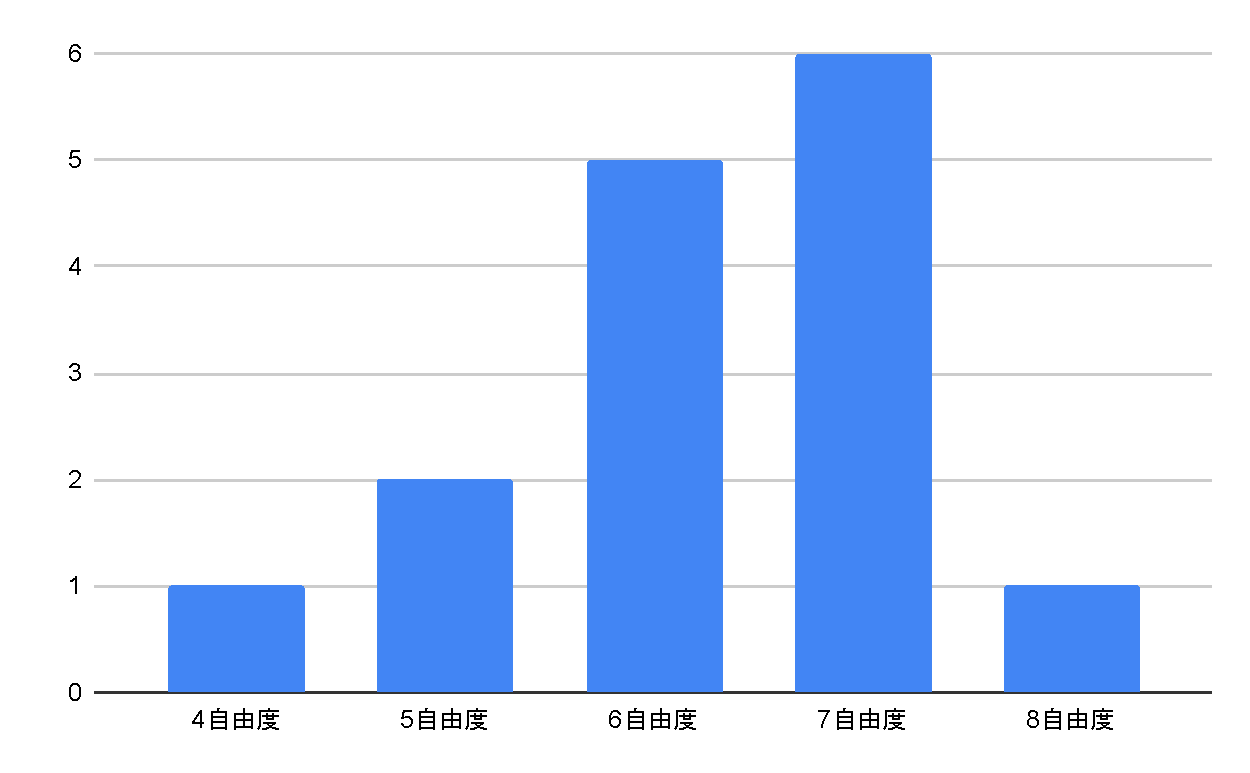
\includegraphics[width=10cm]{images/armDof.pdf}
  \caption{既存のオフィスロボットの自由度}
  \label{fig:armDof}
\end{figure}

\subsection{可搬重量}
設定した作業では、500g以下の対象物を把持する。そのため、アームの可搬重量は500g以上であることが望ましい。
\subsection{エンドエフェクタ}
既存のオフィスロボットのエンドエフェクタは、Mobile ALOHAに搭載されているロボットアーム(\ref{fig:alohaarm}に示す)のような平行グリッパが多く、様々な形状の物体を把持していることが確認できた。そのため、本研究で開発するアームにも平行グリッパを搭載する。

\begin{figure}[h]
  \centering
  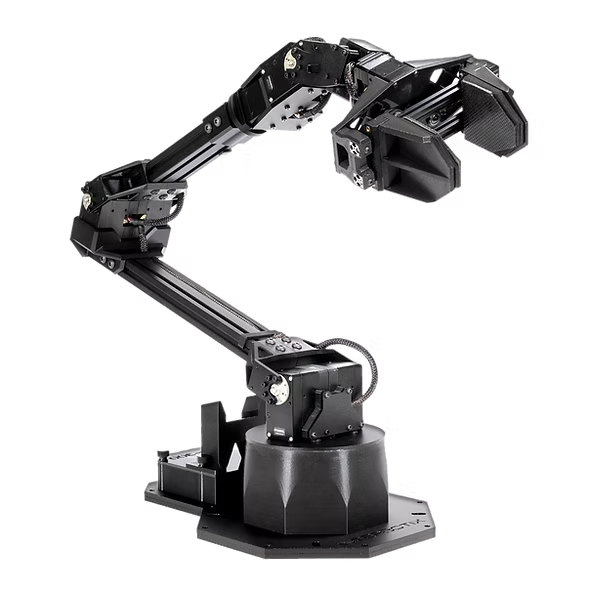
\includegraphics[width=10cm]{images/alohaarm.png}
  \caption{Mobile ALOHO Arm}
  \label{fig:alohaarm}
\end{figure}

\newpage